\documentclass[main.tex]{subfiles}
\begin{document}
\chapter{Appendices for Chapter~\ref{chapter:fame1}}
\label{appendix:fame1}

\section{Azimuthal angle $\phi_{ij}$ calculation}\label{appendix:fame1_phi}
To calculate the azimuthal angle $\phi_{ij}$ for a pair of particle momenta $p_i$ 
and $p_j$ we first consider the plane perpendicular to the momentum 
\begin{eqnarray}\label{eq:pij}
    \vec{p}_{ij} = \vec{p}_{i} + \vec{p}_{j} \, .
\end{eqnarray}
We project the unit vector in the $z$ direction and the momentum of particle $i$ onto 
this plane\footnote{using particle $j$ instead results in a shift of $\phi_{ij}$ by 
$\pi$ which makes no difference for $\sin2\phi$ or $\cos2\phi$.}: 
\begin{eqnarray}\label{eq:north_east}
    \vec{r}_{z} &=& \vec{e}_{z} - \left(\dfrac{\vec{p}_{ij} \cdot \vec{e}_{z}}{\vec{p}_{ij}^{2}}\right) \vec{p}_{ij} \, , \\
    \vec{r}_{i} &=& \vec{p}_{i} - \left(\dfrac{\vec{p}_{ij} \cdot \vec{p}_{i}}{\vec{p}_{ij}^{2}}\right) \vec{p}_{ij} \,.
\end{eqnarray}
The angle $\phi_{ij}$ is the angle between these two projected vectors.
\begin{eqnarray}\label{eq:sin_cos}
    \sin{\phi_{ij}} = 
    \hat r_{ij}\cdot\left( \hat{r}_{i} \times \hat{r}_{z} \right)\, , \quad \cos{\phi_{ij}} = \hat{r}_{i} \cdot \hat{r}_{z} \, ,
\end{eqnarray}
where we have normalised all vectors to be unit vectors:
\begin{equation}
\hat r_z = \frac{\vec{r}_z}{|r_z|}\;, \qquad \hat r_i = \frac{\vec{r}_i}{|r_i|}\;, \qquad \hat r_{ij} = \frac{\vec{p}_{ij}}{|p_{ij}|}\;.
\end{equation}

\section{Jensen's Inequality}\label{appendix:fame1_jensen}
Jensen's inequality states that for concave functions
\begin{eqnarray}
    f(\mathbb{E}[Y]) \geq \mathbb{E}[f(Y)] \, ,
\end{eqnarray}
where $\mathbb{E}$ is the expectation value, the function $f$ in our case is $\mathrm{arcsinh}$ that behaves similarly to the natural logarithm due to the scale of the problem, and $Y$ is a random variable representing our target distribution.
This inequality can be rewritten as
\begin{eqnarray}
    f(\mathbb{E}[Y]) - \mathbb{E}[f(Y)] \geq 0 \, ,
\end{eqnarray}
which is known as Jensen's gap.
With a concave function, the mean of the transformed target distribution will always be underestimating the actual mean, i.e.
\begin{eqnarray}
    \mathbb{E}[Y] \geq \sinh{(\mathbb{E}[\mathrm{arcsinh}{(y)}])} \, ,
\end{eqnarray}
where the LHS is the actual expectation value (cross-section) of the random variable $Y$ and the RHS is the shifted expectation value that the neural network learns.
In our scenario the neural network reduces the variance of the residual distribution, meaning the gap in reality is small but there will always be an offset in the mean value learnt.

\section{Phase-space trajectories}\label{appendix:fame1_trajectory_generation}
We can see the {\RAMBO} algorithm as a map from the unit hypercube in some high dimension into the $n$-particle phase-space. A flat distribution in the hypercube maps to a flat distribution in the multi-particle phase-space. 
To generate our phase-space trajectories we pick two points at random in the unit hypercube and map the line between them using the {\RAMBO} mapping. As a result, each point on the resulting trajectory has equal probability density in phase-space. 
Any other phase-space generator that smoothly maps the unit hypercube to a multi-particle phase-space could replace {\RAMBO} in this procedure and could lead to trajectories with very different characteristics. One could for example imagine a 
sophisticated algorithm that only maps points close to the boundary of the hypercube to soft or collinear configurations. Using such an algorithm would have trajectories that avoid configurations with many particles more collinear or soft than 
the end-points of the trajectories. We find that with {\RAMBO} the trajectories tend not to avoid difficult phase-space configurations and are therefore a good test of the extrapolation properties of our method.

Figure~\ref{fig:detectorpath} shows the trajectory we chose in Section~\ref{sec:trajectories}.

\begin{figure}
    \centering
    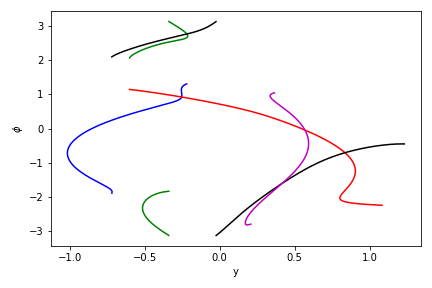
\includegraphics[width=0.45\textwidth]{fame1/yphi.png}
    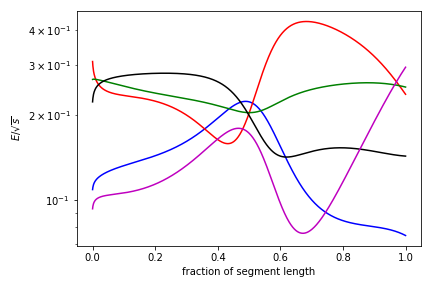
\includegraphics[width=0.45\textwidth]{fame1/E.png}
    \caption{Left: rapidity and azimuthal angle trajectories for the five final state particles in the trajectories used in Section~\ref{sec:trajectories}.
    Right: Evolution of the same particle energies as a function of the position along the segment between the two random points in the unit hypercube.
    }
    \label{fig:detectorpath}
\end{figure}

Here we present another random phase-space trajectory similar to the one
in Figure~\ref{fig:random_trajectory} to demonstrate that features of that
figure are not unique.
\begin{figure}
    \includegraphics[width=\linewidth]{fame1/trajectory_1255.pdf}
    \caption{Another random phase-space trajectory where the `double+single'
    regions of phase-space are explicitly shown in blue.}
    \label{fig:trajectory_1255}
\end{figure}
\end{document}